\chapter{Avaliação do OpenAUTOS}

Neste capítulo são apresentados os experimentos realizados para avaliar o funcionamento do SOE OpenAUTOS.

\section{Testes e Validação}

Para realizar a validação do SO, foi idealizado um circuito sem entradas e com apenas \criarSigla[Diodos Emissores de Luz]{Light-Emitting Diode}{LED}s para saída de dados, utilizados para demostrar o escalonamento das tarefas presentes no SO através de seus acionamentos.

O circuito foi projetado no software de simulação e design de \criarSigla[Placas de Circuito Impresso]{Printed Circuit Board}{PCB} Proteus, versão 8.5, da \emph{Labcenter Electronics Ltd}. Uma versão física deste mesmo circuito foi construída em uma \emph{Protoboard}. Para a obtenção dos resultados nesta versão, utilizou-se um osciloscópio, modelo TDS 2024C, da Tektronix. Ambas versões do circuito podem ser visualizadas na \reffig{cap5_circuit_proteus} e \reffig{cap5_circuit_board}.

\figura{cap5_circuit_proteus}{Circuito no Proteus}{9cm}{}
\figura{cap5_circuit_board}{Circuito na Protoboard}{8cm}{}

Foram realizados um total de 4 experimentos neste circuito, onde 3 deles buscaram validar os diferentes tipos de escalonamento, enquanto que o quarto testou o comportamento do sistema com a alocação de recursos e protocolo prioridade-teto.

Em todos os experimentos, são utilizadas 3 tarefas, responsáveis por fazer os acendimento dos LEDs do circuito. Nas sessões de resultados de seu respectivo experimento, as ondas mostrada pelos osciloscópios representam, respectivamente, as tarefas \texttt{task\_b0}, \texttt{task\_b1} e \texttt{task\_b2}. A \reftab{cap5_osciloscope_color} apresenta uma associação por cores desta relação entre tarefas e ondas dos osciloscópios.

\begin{table}[h]
	\centering
	\caption{Associação das tarefas e cores dos osciloscópios.}
	\label{tab:cap5_osciloscope_color}
	\begin{tabular}{ccc}
		Tarefa            & TDS 2024C & Proteus \\ \hline \hline
		\texttt{task\_b0} & laranja   & amarelo \\ \hline
		\texttt{task\_b1} & ciano     & ciano   \\ \hline
		\texttt{task\_b2} & roxo      & magenta \\ \hline		
	\end{tabular}
\end{table}

\subsection{Experimento 1: Escalonador por Prioridade} \label{cap:cap5_scheduler_p}

O objetivo deste experimento foi o de garantir que o escalonador por prioridades do OpenAUTOS estivesse operando conforme o esperado pela norma, realizando o escalonamento através do uso da chamada das rotinas: \texttt{ActivateTask}, \texttt{TerminateTask} e \texttt{ChainTask}. O código fonte deste experimento pode ser encontrado no \refalg{cap5_scheduler_p_program}, junto de seu arquivo de configuração OIL no \refalg{cap5_scheduler_p_oil}, ambos listados no \refape{capA_validacao}.

\subsubsection{Configuração do Experimento}

Foram utilizadas 5 tarefas, cada qual com um valor único de prioridade, especificadas na \reftab{cap5_scheduler_p}. As funcionalidades de cada tarefa ficaram distribuídas da seguinte maneira:

\begin{table}[h]
	\centering
	\caption{Prioridade das tarefas.}
	\label{tab:cap5_scheduler_p}
	\begin{tabular}{cc}
		Tarefa               & Prioridade \\ \hline \hline
		\texttt{task\_init}  & 254        \\ \hline
		\texttt{task\_start} & 4          \\ \hline
		\texttt{task\_b2}    & 3          \\ \hline
		\texttt{task\_b1}    & 2          \\ \hline
		\texttt{task\_b0}    & 1          \\ \hline
	\end{tabular}
\end{table}

\begin{itemize}
	\item \textbf{\texttt{task\_init}}: única tarefa a iniciar no estado \texttt{READY}, ela faz a inicialização das portas dos sistema, bem como inicia o looping principal de escalonamento entre \textbf{\texttt{task\_start}} e \textbf{\texttt{task\_b\textit{n}}};
	\item \textbf{\texttt{task\_start}}: apaga os LEDs e ativa as tarefas responsáveis por acende-los;
	\item \textbf{\texttt{task\_b\textit{n}}}: acedem o LED respectivo a porta B a qual a tarefa foi associada.
\end{itemize}

Com base nesta configuração, o fluxo de escalonamento do SO pode ser representado no diagrama de estados presente na \reffig{cap5_scheduler_p}.

\figura{cap5_scheduler_p}{Diagrama de estados do escalonador por prioridade}{7cm}{}

\subsubsection{Resultados}

Todas as rotinas testadas agiram conforme a sua especificação. Neste exemplo, a rotina \texttt{ActivateTask} não realizou a chamada a rotina de escalonamento, pois esta deveria escalonar apenas caso estivesse ativando uma tarefa de maior prioridade que a tarefa em execução no momento. O melhor exemplo para este comportamento pode ser visto na tarefa \textbf{\texttt{task\_start}}, que altera os estados das tarefas \textbf{\texttt{task\_b\textit{n}}} de \texttt{SUSPENDED} para \texttt{READY}.

Sendo assim, o escalonamento do sistema passou a ser executado pelas rotinas \texttt{TerminateTask} e \texttt{ChainTask}, que ao realizarem a transição das tarefas do estado \texttt{RUNNING} para \texttt{SUSPENDED}, também fazem uma chamada a rotina de escalonamento. Importante ressaltar que a função \texttt{ChainTask} faz a ativação de uma tarefa antes de se suspender, executando tanto as funções de \texttt{ActivateTask} e \texttt{TerminateTask} em uma única rotina.

A execução destas tarefas podem ser visualizadas nas figuras \ref{fig:cap5_scheduler_p_osc1a} e \ref{fig:cap5_scheduler_p_pro1}.

\figura{cap5_scheduler_p_osc1a}{Escalonador por prioridades - Osciloscópio}{7cm}{}

\begin{figure}[htb]
	\centering
	\caption{Escalonador por prioridades - Proteus.}
	\subfigure[Atraso: $\mu$s]{\label{fig:cap5_scheduler_p_pro1a}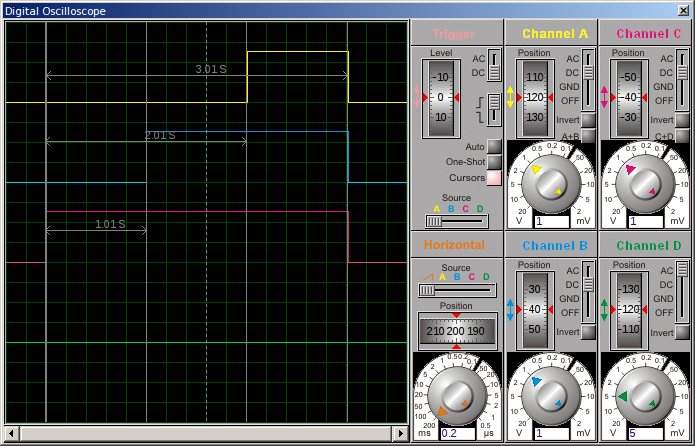
\includegraphics[width=0.45\textwidth]{cap5_scheduler_p_pro1a.png}}
	\subfigure[Atraso: s]{\label{fig:cap5_scheduler_p_pro1b}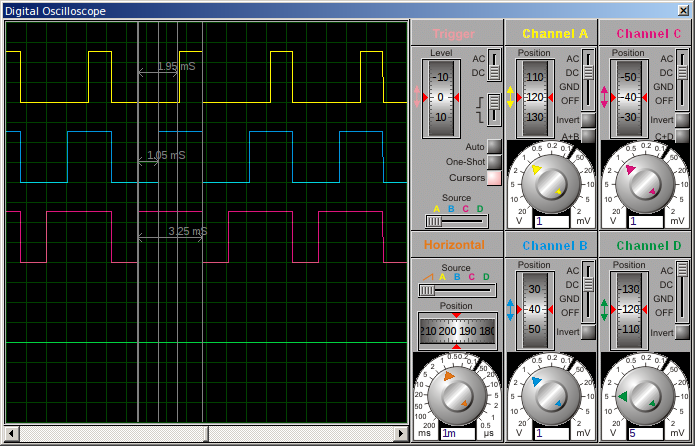
\includegraphics[width=0.45\textwidth]{cap5_scheduler_p_pro1b.png}}
	\label{fig:cap5_scheduler_p_pro1}
\end{figure}

Uma demonstração do circuito em funcionamento pode ser visualizada em \url{https://youtu.be/TBPQiTFyujo}. Para melhor observação do comportamento do sistema foram definidos atrasos de 1 segundo.

\subsection{Experimento 2: Escalonador por Round-Robin}

Diferente do escalonador por prioridades, o escalonamento por \emph{Round-Robin} é realizado por uma interrupção temporal, a qual ocorre apenas quando mais de uma tarefa com a mesma prioridade estejam ativas ao mesmo tempo, podendo estas tarefas serem tanto de tipos diferentes quanto múltiplas ativações de um mesmo tipo. Para fins deste teste, todas as tarefas estão limitadas a apenas uma ativação e são de tipos diferentes, cada qual responsável por um dos LEDs do circuito. O código fonte deste experimento pode ser visualizado no \refalg{cap5_scheduler_rr_program}, junto de seu arquivo de configuração OIL em \refalg{cap5_scheduler_rr_oil}, ambos listados no \refape{capA_validacao}.

\subsubsection{Configuração do Experimento}

Assim como no escalonador por prioridades\refcap{cap5_scheduler_p}, foram utilizadas 5 tarefas, onde uma delas ficou responsável pela inicialização das outras, uma pelo desligamento dos LEDs e as demais pelo acendimento do LED de seu respectivo processo. Diferente do teste anterior, com exceção da tarefa \texttt{task\_init}, nenhuma das outras tarefas encerra sua execução, permanecendo infinitamente ativas, até que o microcontrolador seja desligado.

Como todas as tarefas possuem a mesma prioridade, a ordem de execução se dá exclusivamente pela ordem de ativação das tarefas, conforme especificado pelas linhas 7 à 10 do \refalg{cap5_scheduler_rr_program} do \refape{capA_validacao}. O diagrama de estados presente na \reffig{cap5_scheduler_rr} ilustra a ordem de execução destas tarefas.

\figura{cap5_scheduler_rr}{Diagrama de estados do escalonador por Round-Robin}{7cm}{}

\subsubsection{Resultados}

Assim como no teste anterior, o comportamento do sistema foi exatamente como o especificado pela norma. A cada intervalo de $1_{ms}$, valor adotado pelo OpenAUTOS como o intervalo de escalonamento para Round-Robin, ou seja, o valor do quantum, uma interrupção é gerada pelo temporizador do sistema. Durante esta interrupção, faz-se uma busca pela próxima tarefa de mesma prioridade que se encontra ativa\footnote{No estado \texttt{READY}.}, fazendo com que haja uma troca de contexto em caso afirmativo. Importante ressaltar que esta é a única forma encontrada pela norma de troca de contexto em uma interrupção. Nos demais casos, mesmo que uma tarefa seja ativada durante uma interrupção, ela só será considerada no próximo ponto de escalonamento\footnote{Que se resumem as rotinas: \texttt{Schedule}, \texttt{ActivateTask}, \texttt{TerminateTask}, \texttt{ChainTask}, \texttt{SetEvent}, \texttt{WaitEvent} e \texttt{ReleaseResource}.}.

O resultado da execução deste teste, tanto no modelo físico quanto no virtual, pode ser visualizado na \reffig{cap5_scheduler_rr_osc} e na \reffig{cap5_scheduler_rr_pro}.

\figura{cap5_scheduler_rr_osc}{Escalonador por \emph{Round-Robin} - Osciloscópio}{7cm}{}

\figura{cap5_scheduler_rr_pro}{Escalonador por \emph{Round-Robin} - Proteus}{7cm}{}

Uma demonstração do circuito em funcionamento está disponível em \url{https://youtu.be/QC50OuNeoio}. Para uma melhor visualização do experimento foi aumentado para $1_s$ o tempo de interrupção para chamada do escalonador \emph{Round-Robin}.

\subsection{Experimento 3: Escalonador por Prioridade e Round-Robin}

Este experimento teve como objetivo avaliar o funcionamento do SO em um cenário onde ambos os modelos de escalonamento seriam requisitados. O código para este experimento está disponibilizado no \refalg{cap5_scheduler_prr_program} bem como no arquivo de configuração OIL em \refalg{cap5_scheduler_prr_oil}, ambos listados no \refape{capA_validacao}.

\subsubsection{Configuração do Experimento}

Foram utilizados 5 tipos de tarefas, os quais ficaram organizados da seguinte maneira:

\begin{itemize}
	\item \textbf{\texttt{task\_init}}: tarefa com a menor prioridade, e a única que nunca é encerrada. Ela tem por objetivo manter o programa em ciclo após o encerramento de todas as tarefas de maior prioridade que ela;
	\item \textbf{\texttt{task\_start}}: ativada pela tarefa \textbf{\texttt{task\_init}}, seu papel é o de apagar os LEDS, bem como o de ativar as tarefas que os reacenderão;
	\item \textbf{\texttt{task\_b\textit{n}}}: são as tarefas responsáveis pelo acendimento de seu respectivo LED. Todas possuem a mesma prioridade e também fazem uso a uma chamada na rotina de atraso, para permitir que o tempo de escalonamento do \emph{Round-Robin} execute pelo menos uma vez para cada uma destas tarefas.
\end{itemize}

A \reffig{cap5_scheduler_prr} apresenta um diagrama de estados deste teste, com os seguintes destaques:

\begin{itemize}
	\item Em cinza encontram-se as tarefas que são escalonados pelas rotinas de prioridade;
	\item Em rosa encontram-se as tarefas que possuem mesma prioridade e que são escalonadas por \emph{Round-Robin};
	\item Em preto encontram-se as setas indicando transições que ocorrem exclusivamente por \texttt{TerminateTask};
	\item Em azul encontram-se as setas indicando transições que ocorrem tanto por interrupção quanto por \texttt{TerminateTask};
\end{itemize}

\figura{cap5_scheduler_prr}{Diagrama de estados do escalonador por Prioridade e Round-Robin}{7cm}{}

\subsubsection{Resultados}

O experimento se comportou conforme o esperado onde, em um primeiro momento, o sistema faz a ativação das tarefas através de chamadas a rotina \texttt{ActivateTask}, até então escalonando apenas pela tarefa de maior prioridade ativa na ocasião, que pela lógica do programa acontece na seguinte ordem: \texttt{task\_init}, \texttt{task\_start} e \texttt{task\_b0}.

No momento em que \texttt{task\_b0} entra em execução, apenas tarefas de prioridade idêntica estão ativas no sistema. A partir deste momento, o sistema passa a escalonar as tarefas por \emph{Round-Robin} nos intervalos de quantum definidos pelo SO. O sistema permanece, então, neste modelo de escalonamento até que as tarefas terminem seu tempo de atraso, encerrando, prematuro ao quantum, seu funcionamento através da rotina \texttt{TerminateTask}.

Uma vez encerrada a última das tarefas de ativação de LEDs, a tarefa \texttt{task\_init} volta a ser a tarefa de maior prioridade no sistema, reiniciando o processo.

As ondas dos osciloscópios das figuras \ref{fig:cap5_scheduler_prr_osc} e \ref{fig:cap5_scheduler_prr_pro} ilustram o momento em que as tarefas de acionamento dos LEDs são iniciadas e o tempo no qual elas permanecem processando a rotina de atraso.

\figura{cap5_scheduler_prr_osc}{Escalonador por prioridade e \emph{Round-Robin} - Osciloscópio}{7cm}{}

\figura{cap5_scheduler_prr_pro}{Escalonador por prioridade e \emph{Round-Robin} - Proteus}{7cm}{}

Um vídeo demonstrativo do funcionamento deste circuito encontra-se disponível em \url{https://youtu.be/LSDL_LMfO3o}, também utilizando atrasos de $1_s$ para permitir uma melhor observação do fluxo de funcionamento.

\subsection{Experimento 4: Alocação de Recursos}

Assim como no modelo de prioridade com \emph{Round-Robin}, este experimento utilizou um cenário bem semelhante, porém, com o uso da alocação de recursos e prioridade-teto para que um processo de baixa prioridade pudesse ativar tarefas de maior prioridade sem ser escalonado imediatamente. O código fonte deste experimento pode ser encontrado em \refalg{cap5_scheduler_res_program}, junto de seu arquivo de configuração OIL em \refalg{cap5_scheduler_res_oil}, ambos listados no \refape{capA_validacao}.

\subsubsection{Configuração do Experimento}

Diferente dos outros experimentos, foram utilizadas apenas 4 tarefas, onde:

\begin{itemize}
	\item \textbf{\texttt{task\_init}}: além de fazer a inicialização das portas utilizadas, também é responsável por apagar os LEDs e ativar as tarefas que os reacenderão. Por possuir uma prioridade inferior a das tarefas dos LEDs, \textbf{\texttt{task\_init}} primeiro aloca um recurso de maior prioridade que as tarefas antes de ativá-las. Por fim, esta tarefa é escalonada assim que tem sua prioridade restaurada ao normal, logo após a chamada a rotina \emph{ReleaseResource}. este processo de alocação do recurso pode ser visualizado no diagrama de sequência na \reffig{cap5_scheduler_res};
	\item \textbf{\texttt{task\_b\textit{n}}}: tarefas que realizam o acendimento dos LEDS.
\end{itemize}

\figura{cap5_scheduler_res}{Diagrama de sequencia da alocação de recurso e prioridade-teto}{7cm}{}

\subsubsection{Resultados}

Após a alocação do recurso, a tarefa \texttt{task\_init} passou a ter uma prioridade superior a das tarefas que estaria ativando, permitindo que ativasse todas as tarefas \texttt{task\_b\textit{n}} sem que ela própria fosse escalonada.

A partir do momento no qual o recurso alocado por \texttt{task\_init} é liberado, esta tem sua prioridade reduzida para seu valor original, o qual é inferior ao das demais tarefas que se encontram aptos para execução. Sendo assim, o SO passa a executar as tarefas de maior prioridade, que por possuírem valores idênticos de prioridade, são escalonados por \emph{Round-Robin} até que sua execução encerre com a chamada a rotina \emph{TerminateTask}, reiniciando o clico em \texttt{task\_init}.

Caso \texttt{task\_init} tentasse ativar as demais tarefas sem antes ter feito a alocação do recurso, o SO teria interrompido seu processamento ao retornar da rotina \emph{ActivateTask}, executando cada tarefa até seu encerramento em \emph{TerminateTask}, sem nunca escalonalas por \emph{Round-Robin}.

Os resultados da execução deste experimento podem ser vistos nos gráficos da \reffig{cap5_scheduler_res_osc} e \reffig{cap5_scheduler_res_pro}.

\figura{cap5_scheduler_res_osc}{Alocação de recurso e prioridade-teto - Osciloscópio}{7cm}{}

\figura{cap5_scheduler_res_pro}{Alocação de recurso e prioridade-teto - Proteus}{7cm}{}

Um vídeo demonstrativo do funcionamento deste circuito encontra-se disponível em \url{https://youtu.be/XbD-STWvOCU}, também utilizando atrasos de $1_s$ para permitir uma melhor observação do fluxo de funcionamento.

\section{Dificuldades}

Diversas foram as dificuldades encontradas para o desenvolvimento deste projeto. Na sequência serão descritas algumas delas.

\subsection{Geração de Instruções Defeituosas pelo Compilador XC8}

Por razões desconhecidas, a instrução \texttt{movff}, em Assembly, muitas vezes não realizava nenhuma ação, principalmente quando utilizada com alguns registradores especiais, como os \texttt{TOSU}, \texttt{TOSH} e \texttt{TOSL}, utilizados para manipulação da pilha dos microcontroladores da linha PIC18F, bem como os registradores \texttt{TMR0} e \texttt{TMR1}, utilizados para calcular o tempo de estouro de seus respectivos temporizadores\footnote{Escrever um valor literal nestes registradores sempre resulta em um código operante, pois o compilador passa a utilizar o comando \texttt{movlf} ao invés de \texttt{movff}.}.

Esta instrução é automaticamente utilizada pelo compilador XC8 e, na maioria dos casos, funciona corretamente. Infelizmente, para estes casos onde ela não funcionou, foi necessário que uma parte de código Assembly fosse escrito manualmente para contornar o seu uso.

\subsection{Seleção de Bancos de Memória}

Devido a grande quantidade de memória alocada estaticamente pelo OpenAUTOS e tarefas definidas pelo usuário, um dos inconvenientes que passou a ser notado foram as indicações de bancos de memória cheios.

Idealmente, ele deveria ser capaz de declarar estas variáveis que excederiam o limite de um banco de memória em um outro banco automaticamente. Porém, o compilador não estava realizando esta operação, que teve que ser realizada manualmente a partir de instruções Assembly.

Um outro inconveniente que passou a ser observado foi a má distribuição dos espaços presentes nos bancos de memória do microcontrolador, o que pode ser notado no arquivo de extensão \emph{lst} gerado durante a compilação da imagem do hardware, onde há diversas segmentações de memória e a maioria dos bancos apresentam um espaço considerável ainda.

Por este projeto utilizar apenas a versão gratuita do compilador, e também por ter suas compilações apenas em modo de \emph{Debug}, acredita-se que diversas otimizações ainda possam ser alcançadas neste quesito.

\subsection{Ferramentas de Depuração}

Embora de grande ajuda na depuração de \emph{bugs}, algumas vezes as ferramentas MPLAB e Proteus não conseguem acompanhar perfeitamente os formatos de imagem para depuração suportados pelo compilador XC8, que são o \emph{elf} e \emph{cof}, o que acaba forçando o desenvolvedor a buscar meios alternativos de buscar informações em uma determinada área de código, geralmente resultando no uso de LEDs para indicar estados do sistema.

\subsection{Abrangência da Norma}

Mesmo com a alta disponibilidade de informações sobre projetos e artigos que atuam nas normas do OSEK/VDX e AUTOSAR, pouquíssimos são aqueles se aprofundam nos temas. Isto implica que a maior parte das informações devem ser extraídas diretamente das normas, o que passa a ser um processo trabalhoso devido a extensão e complexidade das mesmas.

É, também, difícil de acompanhar e levantar todos os detalhes referentes a cada módulo proposto, já que as normas costumam separar informações entre elas que complementam estes sistemas.
